\documentclass[a4paper, 12pt]{article}

\usepackage{babel}
\usepackage{enumitem}
\usepackage{times}
\usepackage{graphicx}
\usepackage{geometry}
	\geometry{left = 4cm, top = 4cm, right = 3cm, bottom = 3cm}
\usepackage{float}
\usepackage{setspace}
	\setstretch{1.5}
\usepackage{listings}
\usepackage{hyperref}


\begin{document}
\title{\huge\textbf{TUGAS BESAR DATABASE II\\
Cara Membuat Aplikasi Sistem Penjualan Pakaian Akhwat}}
\date{}

\maketitle




\begin{center}
\vspace{2cm}
Mauliddhia Restu Shafina\\
D4 TI 2C\\
1.18.4.101\\
\vspace{4cm}
\textbf{PROGRAM DIPLOMA IV POLITEKNIK POS INDONESIA} \linebreak
\textbf{POLITEKNIK POS INDONESIA} \linebreak
\textbf{BANDUNG}\linebreak
\textbf{2019}\\

\end{center}

\section{Langkah Kerja}
\begin{enumerate}

\item Buka google, lalu cari “Oracle Apex Online” . Setelah itu pilih sign in jika sudah pernah mendaftar dan jika belum pernah mendaftar maka daftar dengan mengisi data-data yang diminta pada pendaftaran apliaksi Oracle Apex Online itu.

\item Setelah memiliki akun maka klik \textit{sign in} lalu isi \textit{workspace, username} dan \textit{password} pada oracle apex online.

            \begin{figure}[!htbp]
            \centering
            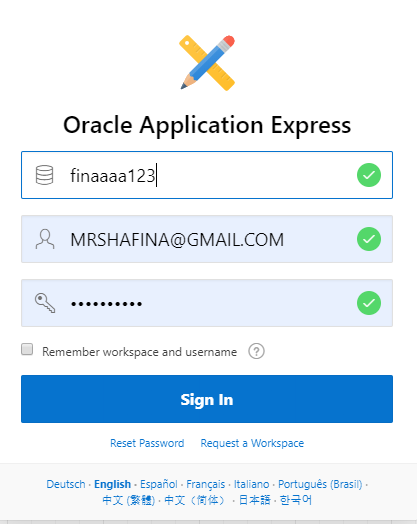
\includegraphics[width=6cm,height=7cm]{gambar/1.PNG}
            \caption{Tampilan Awal jika akan sign in pada Oracle Apex}
            \label{penanda}
            \end{figure}

\item Jika sudah masuk pada Oracle Apex, maka pilih salah satu menu pada Oracle Apex yaitu SQL workshop, dan pilih SQL Command.

            \begin{figure}[!htbp]
            \centering
            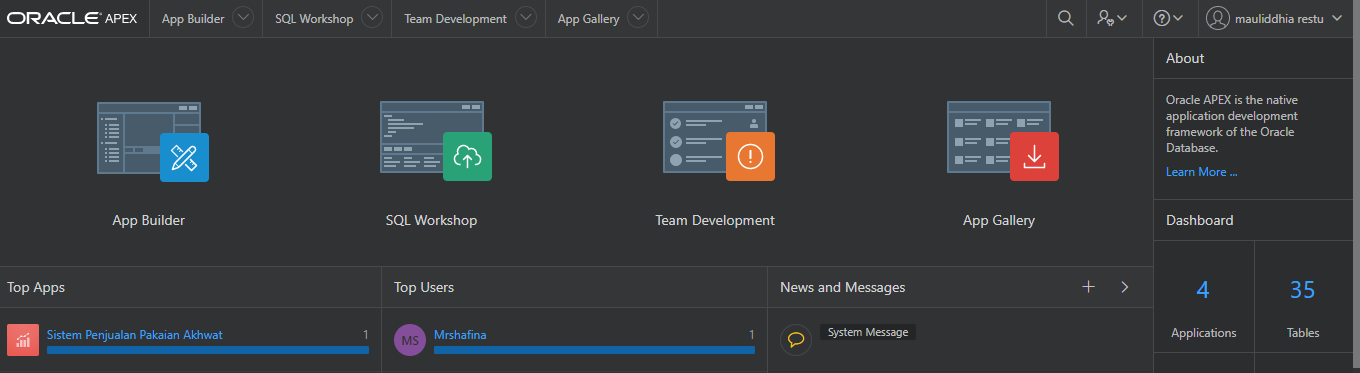
\includegraphics[width=10cm,height=4cm]{gambar/tampilanmenu.PNG}
            \caption{Tampilan Utama pada Oracle Apex}
            \label{penanda}
            \end{figure}
            
\item SQL Command itu sendiri adalah tempat untuk membuat codingan. Nah, sebelum membuat aplikasi saya membuat tabel yang saya butuhkan untuk aplikasi terlebih dahulu.
\subsection{Membuat tabel penjualan}
Pertama saya membuat tabel Penjualan. Pada tabel penjualan saya membuat kolom yang berisi Kode Penjualan ( Sebagai Primary Key dari tabel Penjualan), id barang(Foreign Key), id pegawai (Foreign Key), jumlah barang, sisa stok, tanggal penjualan, dan harga total. berikut codingannya. 

            \begin{figure}[!htbp]
            \centering
            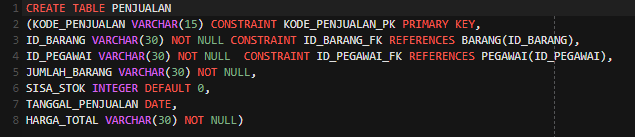
\includegraphics[width=10cm,height=2cm]{gambar/c-1.PNG}
            \caption{Codingan membuat tabel Penjualan}
            \label{penanda}
            \end{figure}\\
            
Kedua, saya membuat tabel Barang. Pada tabel barang saya membuat kolom yang berisi id barang (Primary Key), nama barang, harga beli, harga jual, jumlah awal, dan terjual.Berikut codingannya.

            \begin{figure}[!htbp]
            \centering
            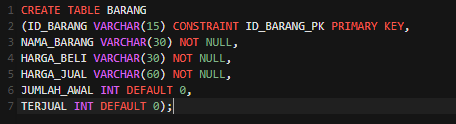
\includegraphics[width=10cm,height=2cm]{gambar/c-2.PNG}
            \caption{Codingan membuat tabel Barang}
            \label{penanda}
            \end{figure}\\

Ketiga, saya membuat tabel Pegawai. Pada tabel pegawai saya membuat kolom yang berisi id pegawai(Primary Key), nama pegawai, dan alamat pegawai.

            \begin{figure}[!htbp]
            \centering
            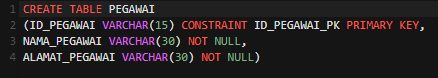
\includegraphics[width=10cm,height=2cm]{gambar/c-3.PNG}
            \caption{Codingan membuat tabel Pegawai}
            \label{penanda}
            \end{figure}\\
            
\subsection{Mengisi Tabel}
\par Setelah membuat tabel, kita isi tabel itu satu per satu. \\
Pertama kita mengisi tabel Penjualan terlebih dahulu dengan codingan seperti dibawah ini.

            \begin{figure}[!htbp]
            \centering
            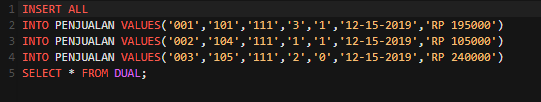
\includegraphics[width=10cm,height=4cm]{gambar/1-insert.PNG}
            \caption{Codingan Mengisi Tabel}
            \label{penanda}
            \end{figure}\\
            
Kedua, kita mengisi tabel Barang sama seperti tabel penjualan. Berikut codingannya. 

            \begin{figure}[!htbp]
            \centering
            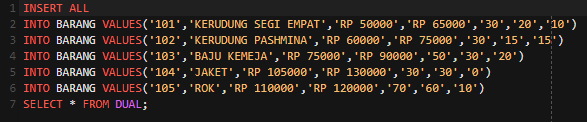
\includegraphics[width=10cm,height=4cm]{gambar/3-insert.PNG}
            \caption{Codingan Mengisi Tabel}
            \label{penanda}
            \end{figure}\\
            
Ketiga, kita mengisi tabel Pegawai. Berikut codingannya.

            \begin{figure}[!htbp]
            \centering
            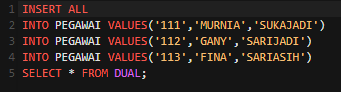
\includegraphics[width=10cm,height=3cm]{gambar/2-insert.PNG}
            \caption{Codingan Mengisi Tabel}
            \label{penanda}
            \end{figure}\\
            
\subsection{Membuat Fungsi Triger}
\par Setelah membuat tabel dan mengisi kolom yang telah dibuat, maka selanjutnya kita membuat fungsi triger pada tabel yang telah dibuat tadi. Triger itu sendiri merupakan fungsi yang digunakan untuk menampilkan suatu data secara otomatis ketika kita menggunakan perintah insert, delete, dan update pada tabel. berikut triger yang telah saya buat.

            \begin{figure}[!htbp]
            \centering
            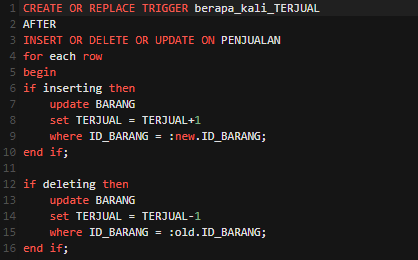
\includegraphics[width=10cm,height=6cm]{gambar/1-Triger.PNG}
            \caption{Tampilan Coding pada Triger 1}
            \label{penanda}
            \end{figure}

            \begin{figure}[!htbp]
            \centering
            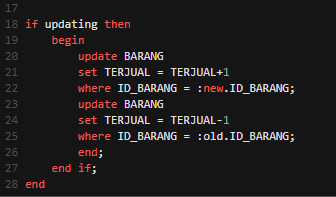
\includegraphics[width=10cm,height=5cm]{gambar/2-Triger.PNG}
            \caption{Tampilan Lanjutan Coding pada Triger 1}
            \label{penanda}
            \end{figure}
            
\par Pada codingan triger diatas saya beri nama "berapa kali terjual", yang di setting menggunakan perintah insert, delete, dan update pada tabel Penjualan yang nantinya akan berubah secara otomatis pada tabel Barang di kolom Terjual.

\subsection{Membuat View}
\par Setelah membuat fungsi triger, kita membuat view. View itu sendiri adalah suatu perintah untuk menggabungkan query join, innerjoin tabel dengan sederhana. Berikut codingan tentang view. 
            
            \begin{figure}[!htbp]
            \centering
            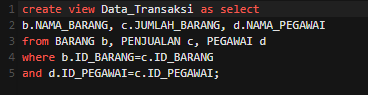
\includegraphics[width=10cm,height=3cm]{gambar/view.PNG}
            \caption{Tampilan Coding pada View}
            \label{penanda}
            \end{figure}

\par Pada view diatas, saya telah memasukkan nama kolom pada tabel yang berbeda yaitu nama barang, jumlah barang, dan nama pegawai. 

\item Setelah semuanya selesai, maka kita membuat aplikasi dengan kembali ke halaman utama dan memilih "App Builder" untuk memulai membuat aplikasi. Seperti gambar di bawah ini 

            \begin{figure}[!htbp]
            \centering
            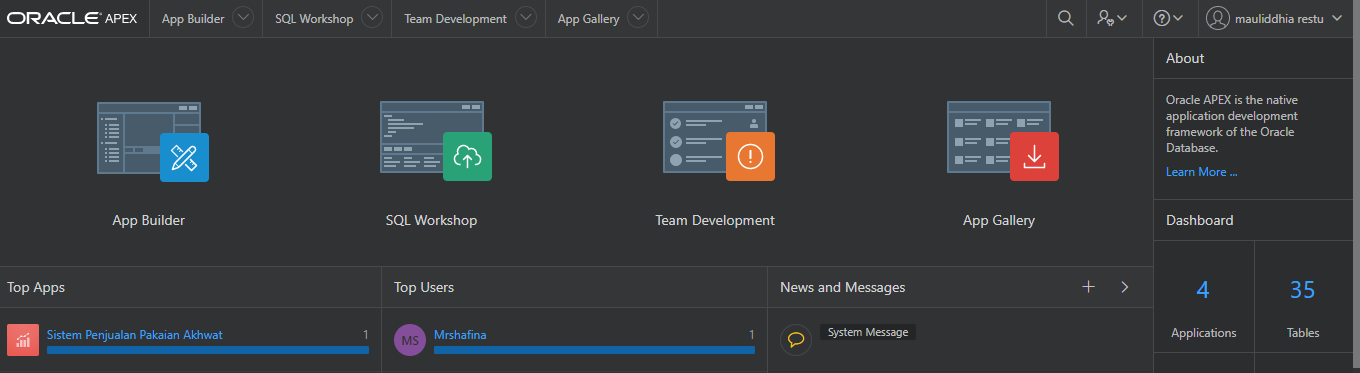
\includegraphics[width=10cm,height=8cm]{gambar/tampilanmenu.PNG}
            \caption{Tampilan Menu Utama pada Oracle Apex}
            \label{penanda}
            \end{figure}

\item Setelah itu, pilih menu Create seperti gambar dibawah ini. 

            \begin{figure}[!htbp]
            \centering
            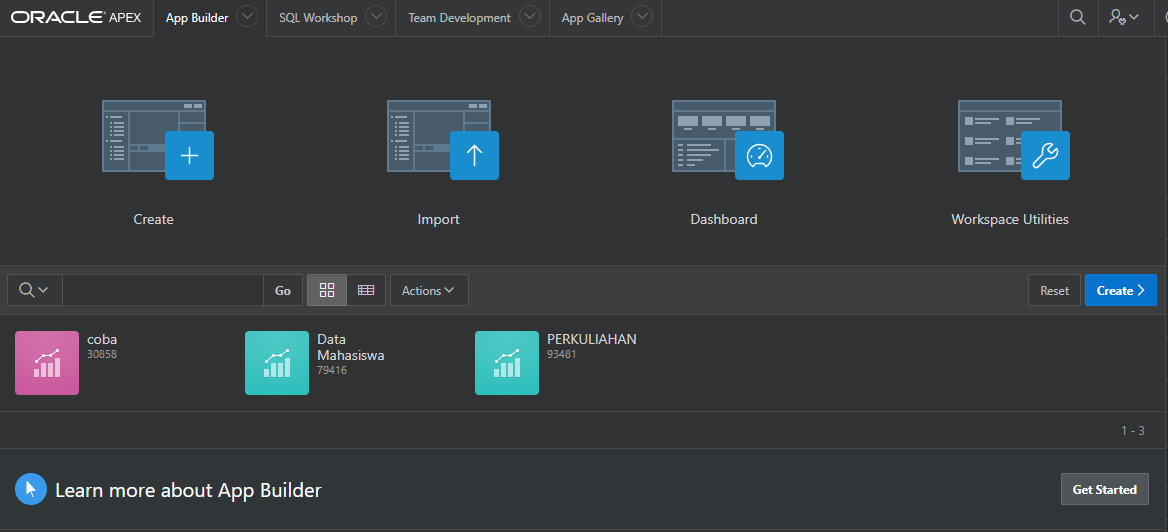
\includegraphics[width=10cm,height=8cm]{gambar/1-createapp.PNG}
            \caption{Tampilan Menu untuk Membuat Aplikasi}
            \label{penanda}
            \end{figure}
            
\par Setelah itu, akan ada tampilan seperti dibawah ini dan kita pilih "New Application" pada gambar dibawah. 

            \begin{figure}[!htbp]
            \centering
            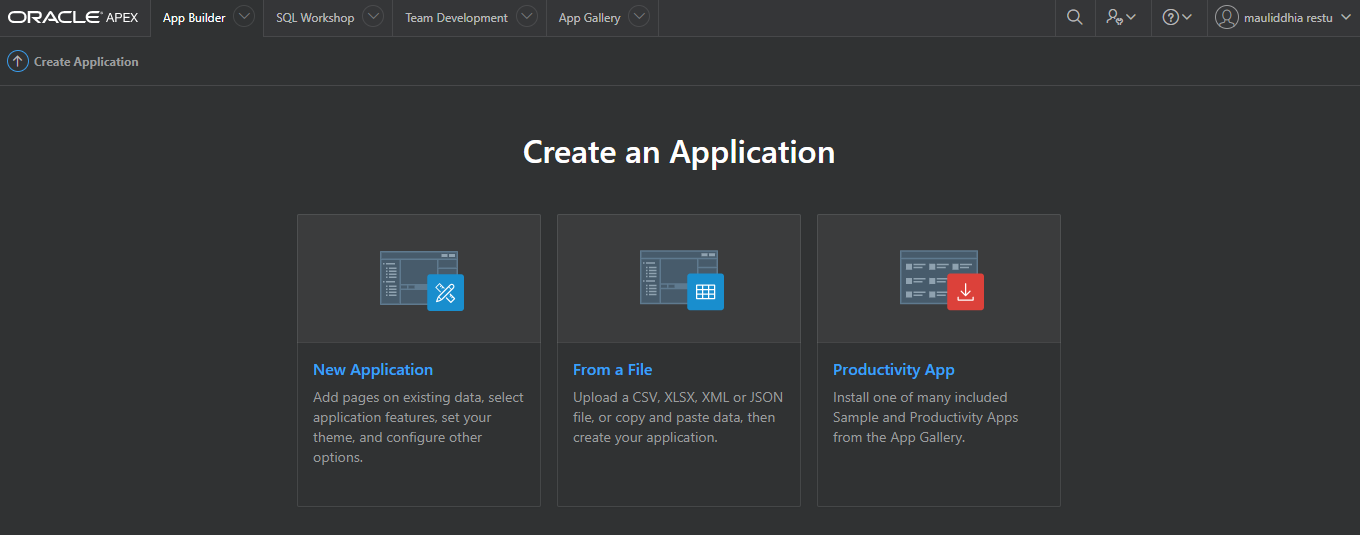
\includegraphics[width=10cm,height=9cm]{gambar/2-createapp.PNG}
            \caption{Tampilan Menu Untuk Membuat Aplikasi }
            \label{penanda}
            \end{figure}

\item Setelah itu, buat nama aplikasi yang akan kita buat. Jika ingin mendesain warna pada halaman aplikasi maka gunakan "Application" yang ada di sebelah kanan "Name" itu. 

            \begin{figure}[!htbp]
            \centering
            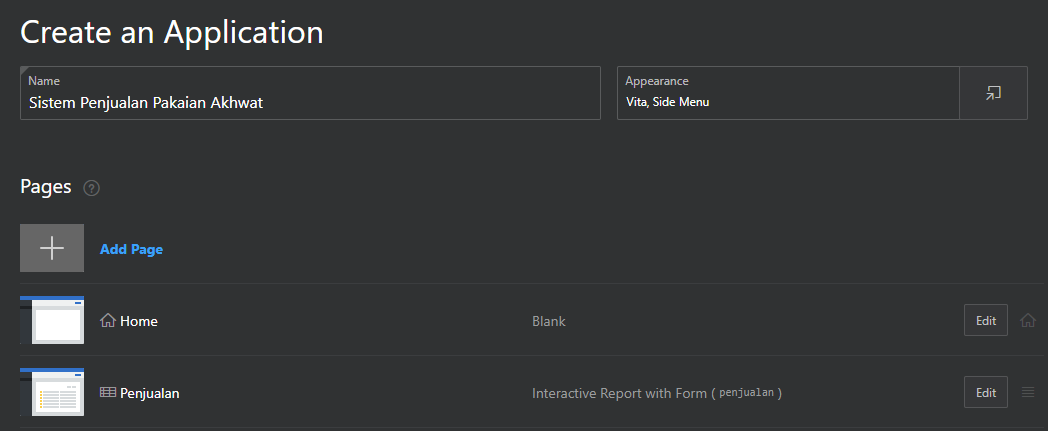
\includegraphics[width=10cm,height=7cm]{gambar/3-createapp.PNG}
            \caption{Tampilan untuk Aplikasi}
            \label{penanda}
            \end{figure}
            
\par Untuk menambah halaman pada aplikasi, kita bisa klik "Add Page". Karena tabel yang kita buat di atas ada tiga, maka kita menambah halaman menjadi tiga. 

            \begin{figure}[!htbp]
            \centering
            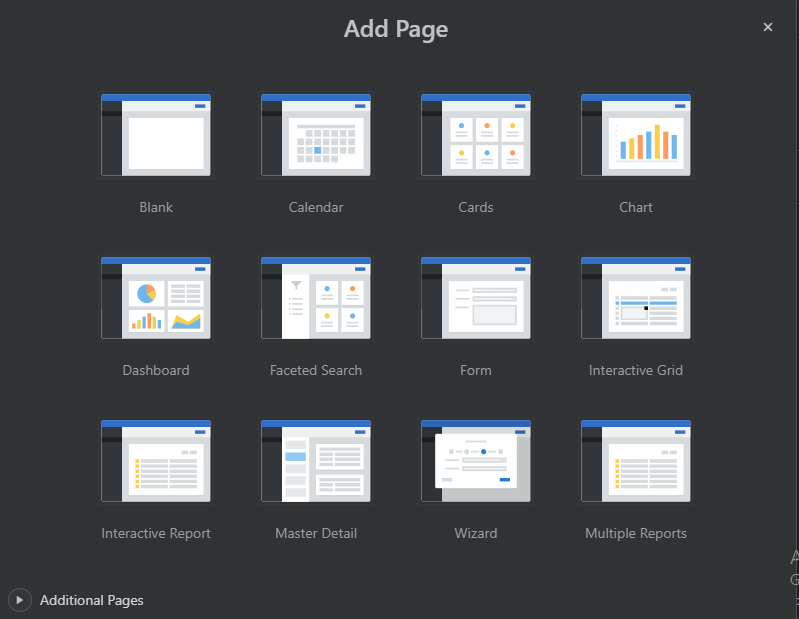
\includegraphics[width=10cm,height=7cm]{gambar/4-createapp.PNG}
            \caption{Tampilan Menu pada Add Page}
            \label{penanda}
            \end{figure}
            
\par Disini saya memilih halaman "Interactive report" lalu akan muncul gambar seperti dibawah yang mengharuskan saya mengisi "Nama Page" dan memilih tabel yang akan di masukkan pada halaman itu. Lakukan yang sama pada tabel Penjualan, Barang, dan Pegawai. Berikut gambarnya.

            \begin{figure}[!htbp]
            \centering
            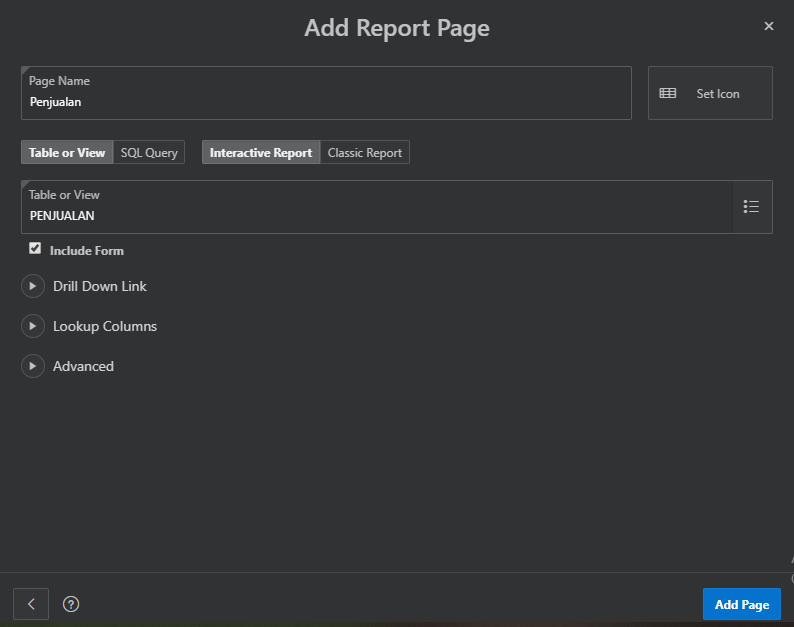
\includegraphics[width=10cm,height=5cm]{gambar/7-createapp.PNG}
            \caption{Tampilan Add Report Page Penjualan}
            \label{penanda}
            \end{figure}
            
            \begin{figure}[!htbp]
            \centering
            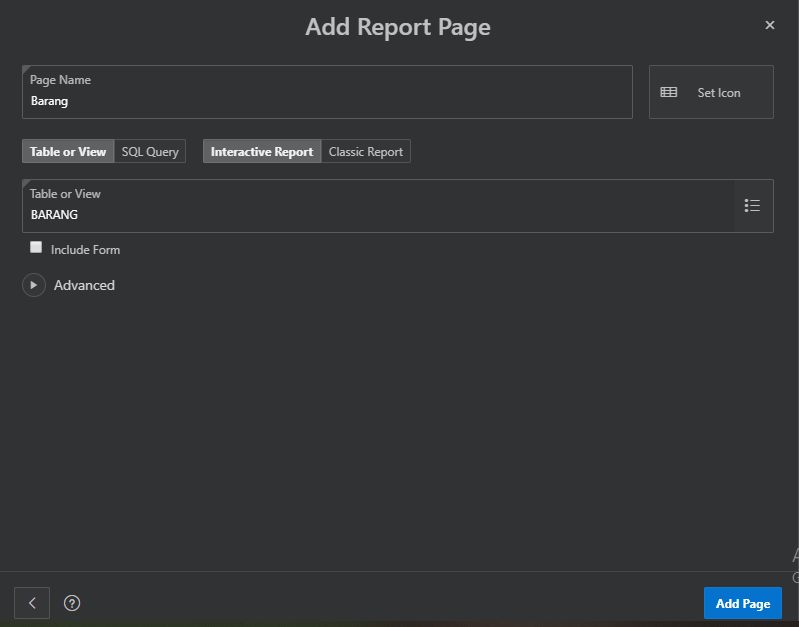
\includegraphics[width=10cm,height=5cm]{gambar/5-createapp.PNG}
            \caption{Tampilan Add Report Page Barang}
            \label{penanda}
            \end{figure}
            
            \begin{figure}[!htbp]
            \centering
            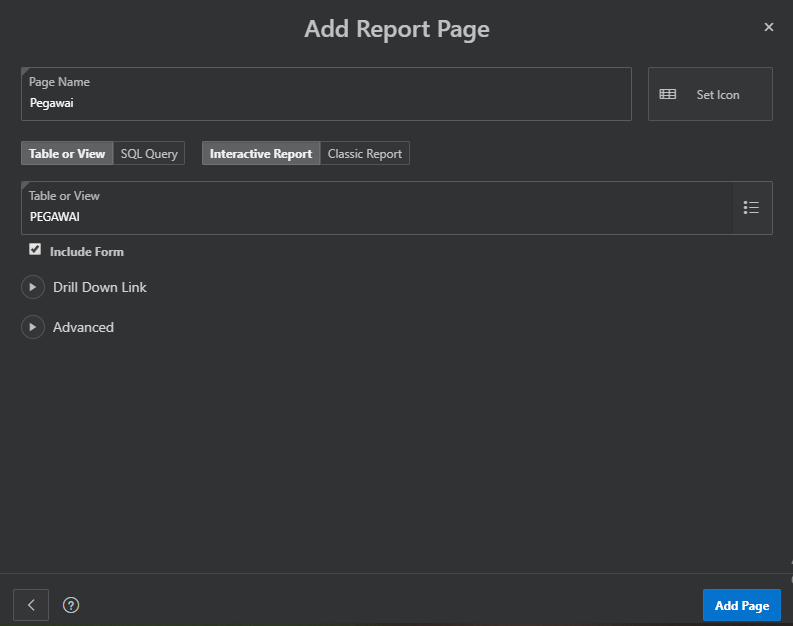
\includegraphics[width=10cm,height=5cm]{gambar/6-createapp.PNG}
            \caption{Tampilan Add Report Page Pegawai}
            \label{penanda}
            \end{figure}
            
\item Setelah menambahkan halaman, dilanjutkan dengan menceklis semua yang ada pada "Features". Jangan lupa untuk meng-klik "Create Application". Seperti pada gambar dibawah ini.

            \begin{figure}[!htbp]
            \centering
            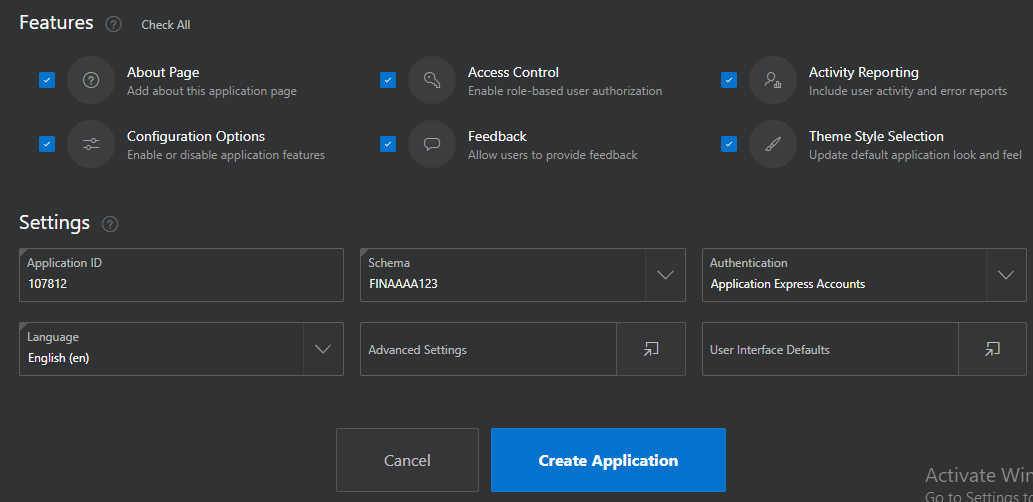
\includegraphics[width=12cm,height=7cm]{gambar/8-createapp.PNG}
            \caption{Tampilan Features}
            \label{penanda}
            \end{figure}
            
\item Setelah itu, akan muncul menu seperti dibawah ini dan klik pilihan "Run Application".

            \begin{figure}[!htbp]
            \centering
            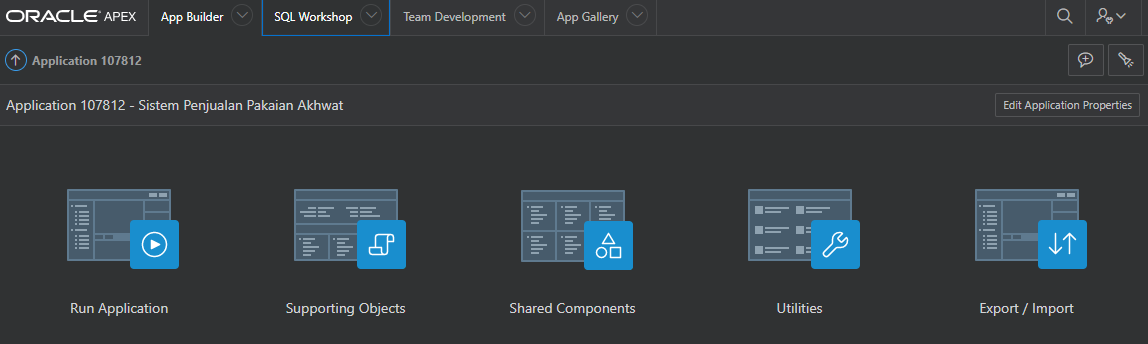
\includegraphics[width=12cm,height=8cm]{gambar/9-createapp.PNG}
            \caption{Tampilan Menu untuk Run Aplikasi}
            \label{penanda}
            \end{figure}
            
\item Akan muncul halaman untuk login pada aplikasi yang tadi telah kita buat. Lihat gambar dibawah.

            \begin{figure}[!htbp]
            \centering
            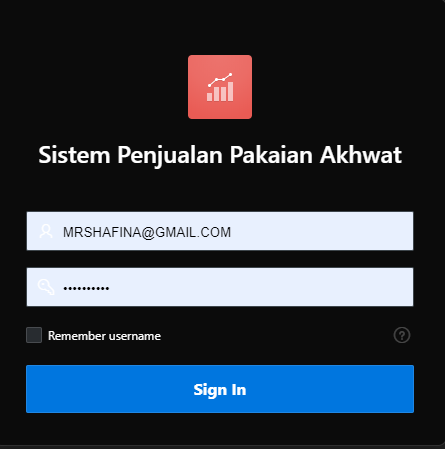
\includegraphics[width=10cm,height=11cm]{gambar/10-createapp.PNG}
            \caption{Tampilan Login pada Aplikasi yang telah dibuat}
            \label{penanda}
            \end{figure}
            
\item Setelah itu, akan muncul halaman aplikasi yang telah kita buat tadi. selesai.

            \begin{figure}[!htbp]
            \centering
            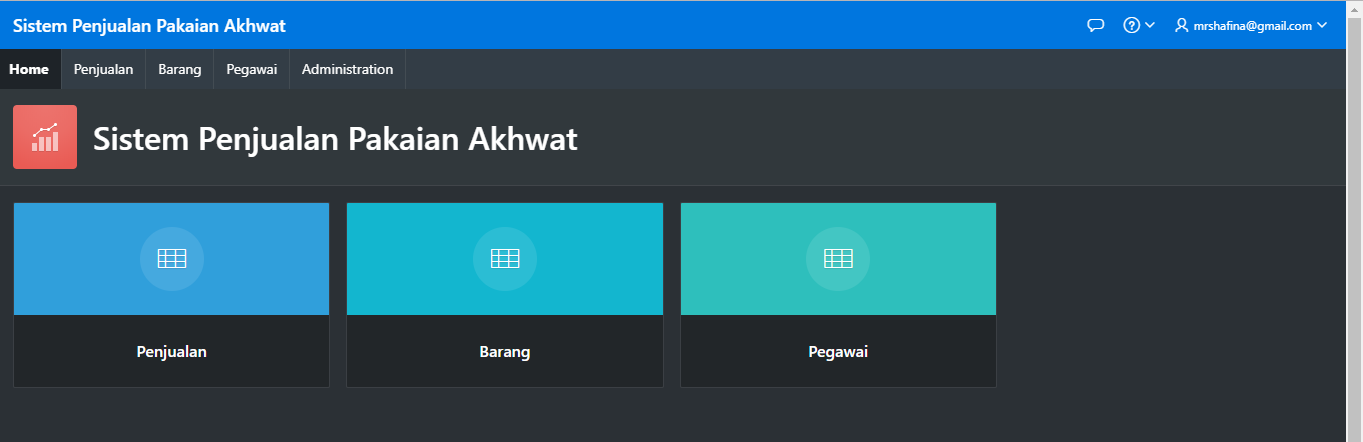
\includegraphics[width=10cm,height=6cm]{gambar/11-createapp.PNG}
            \caption{Tampilan Aplikasi yang telah dibuat}
            \label{penanda}
            \end{figure}
 
\item \url{https://apex.oracle.com/pls/apex/f?p=107812:LOGIN_DESKTOP:701232253842554:::::}\\
Username  : mrshafina@gmail.com\\
Password  : finaaaa123\\
Workspace : FINAAAA123

\end{enumerate}




\end{document}

